\documentclass[]{ltugboat}
\interlinepenalty=-500
\usepackage[utf8]{inputenc}
\usepackage[T2A,T1]{fontenc}
\usepackage{graphicx}
\usepackage[breaklinks,colorlinks,linkcolor=black,citecolor=black,
            urlcolor=black]{hyperref}
\begin{document}
\title{Paragraph designer with galley approach}
\author{Oleg Parashchenko}
\address{bitplant.de GmbH\\
Fabrikstr. 15\\
89520 Heidenheim, Germany}
\netaddress{olpa (at) uucode dot com}
\personalURL{http://uucode.com/}
\maketitle

\begin{abstract}
The \LaTeX{} package \verb|paravesp| controls the space above and below paragraphs.

The python script \verb|parades.py| generates paragraph styles with support of space above, space below and tabulators.

The system imposes the galley approach on the document.
\end{abstract}

\section{Introduction}

One layout specification defined the space above and below paragraphs. This is not how does \TeX{} work. To satisfy the requirement, the package \verb|paravesp| (\acro{PARA}graph \acro{VE}rtical \acro{SP}ace) was developed.

The solution imposes the galley approach on the document. The paragraphs should be wrapped by a tracking code, which controls how the matherial is added into the \TeX{} vertical list.

The paragraph designer appeared as a generalization of the tracking code to other paragraph properties. The user describes the formatting options in a python file. The program \verb|parades.py| converts the definitions into \TeX{} code.

The system successfully works in the production, but so far is limited to my needs. The complete set of the paragraph properties is not a momentary goal. A switch to the package \verb|xgalley| from the \LaTeX{}3 project might be a step in the future development.

The article starts with the definition what the space between paragraphs is and how it is implemented. The example demonstrates the use of the commands, which are then described using pseudocode.

The paragraph designer is first illustrated by a sample \LaTeX{} fragment, which uses the paragraph styles. For each three types of styles, there are given a sample definition in Python and the result of translation to \TeX{} code, with explanation. Finally, the reference lists all the supported paragraph properties and the commands of the Python \verb|parades.py| tool.

The article concludes with information on how to get the code and run it.

\section{Space between paragraphs}

The notion "space between paragraphs" can be defined differently.

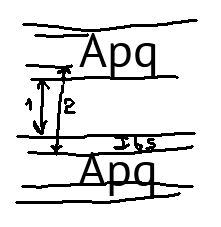
\includegraphics[width=6cm]{betwpara.png}

In one definition, the space between paragraphs is the amount of additional space comparing to what happens inside a paragraph. This is what the most typesetting engines implement, and what is named \verb|parskip| in \TeX{}. If the space between paragraphs is set to zero, \TeX{} still adds space \verb|baselineskip| minus \verb|prevdepth| minus the height of the letters.

The definition of the package \verb|paravesp| is: the space between paragraphs is the distance between the baseline of the preceeding paragraph and the top of the next paragraph. The code cares that this distance is larger than \verb|prevdepth|.

The command \cs{ParaSpaceAbove}, which preceedes a paragraph, can't know how much glue induced by \verb|baselineskip| will be added. Therefore, the command disables this glue completely by setting \verb|prevdepth| to infinity.

The commands rely on automatic insertion of \verb|parskip| glue by \TeX. This insertion doesn't happen if the next element in the vertical list is not a paragraph but some box. In this case, make the space manually using the command \verb|IssueParaSpace|.

\subsection{Usage}

The package \verb|paravesp| imposes restrictions on how to construct a document. Otherwise it can't guarantee the desired space above or below paragraphs.

\begin{itemize}
\item Switches between the vertical and horizontal modes be controlled. \TeX{} automation is partially forbidden.
\item The register \cs{parskip} belongs to the controlling code.
\end{itemize}

The guidelines for the controlling code are:

\begin{itemize}
\item At the end of a paragraph (after \cs{par}) use the command \cs{ParaSpaceBelow}.
\item At the begin of a paragraph, still in the vertical mode, use \cs{ParaSpaceAbove}.
\item At the begin of a block content, for which \TeX{} will not insert \cs{parskip} automatically, use the both \cs{ParaSpaceAbove} and \cs{IssueParaSpace}.
\end{itemize}

An example:

\begin{verbatim}
...
\ParaSpaceAbove{20pt}%
{\HeadingStyle Heading}\par
\ParaSpaceBelow{20pt}%
\ParaSpaceAbove{10pt}%
An usual paragraph of text...\par
\ParaSpaceBelow{10pt}%
\ParaSpaceAbove{10pt}%
Yet another usual paragraph of text...\par
\ParaSpaceBelow{10pt}%
\ParaSpaceAbove{20pt}\IssueParaSpace
\vbox{\fbox{Some info-box}}%
\ParaSpaceBelow{20pt}%
...
\end{verbatim}

\subsection{Technical details}

Below is the simplified approximation what happens. The special cases are not shown.

\medskip

After \cs{ParaSpaceBelow\{length\}}:

\begin{itemize}
\item vertical list is not changed
\item \verb|parskip| := \textit{length} - \verb|prevdepth|
\item \verb|prevdepth| is not changed
\end{itemize}

The command \cs{ParaSpaceBelow} splits its argument on two lengths, \verb|prevdepth| and \verb|parskip|. This is a precaution for the case if the the next element in the vertical list is not controlled by galley. Thanks to the retained \verb|prevdepth|, a possible layout corruption is avoded.

\medskip

After \cs{ParaSpaceAbove\{length\}}:

\begin{itemize}
\item vertical list: \verb|vskip -prevdepth|,\\penalty as before \verb|vskip|
\item \verb|parskip| := max(\textit{length}, \textit{old\_length})
\item \verb|prevdepth| := -1000pt
\end{itemize}

\medskip

After \cs{IssueParaSpace}:

\begin{itemize}
\item vertical list: \verb|vskip| \verb|parskip|,\\penalty as before \verb|vskip|
\item \verb|parskip| := 0pt
\item \verb|prevdepth| := -1000pt
\end{itemize}

\medskip

After \cs{IgnoreSpaceAboveNextPara}:

\begin{itemize}
\item vertical list is not changed
\item parskip := -0.01pt
\item prevdepth is not changed
\end{itemize}

The special case is \verb|parskip| less than 0pt, which cancels the vertical spacing. It is useful when display content (image, list etc) is the first element inside a table cell.

\section{Paragraph designer}

The paragraph designer transforms Python objects with desired paragraph properties into \TeX{} code which implements these properties.

The main benefit is that the paragraphs definitions can be constructed in such way that the repetitions (for example, font names) can be extracted into common settings.

The system proposes that every block-level element of a document should be wrapped into a command or an environment, which support the galley approach. The suggested sorts of the paragraphs:

\begin{itemize}
\item long body text paragraphs, wrapped by an environment,
\item short paragraphs, wrapped by a command, and
\item short paragraphs with tabstops, also wrapped by a command.
\end{itemize}

The document, made using this approach, looks structured. Here is an example.

\begin{verbatim}
\HeadI{Universal Declaration of Human Rights}
\HeadII{Preamble}
\begin{para}Whereas recognition...\end{para}
\begin{para}Whereas disregard
    and contempt...\end{para}
...
\HeadII{Article 14}
\begin{udhrlist}
\listitem{1}{Everyone has the right ...}
\listitem{2}{This right may not be invoked ...}
\end{udhrlist}
\end{verbatim}

The sample is generated automatically from the \XML{} source. The generation script, the paragraph styles as Python definition and \verb|.sty| result, the result are included by the package in the directory \verb|udhr|.

\subsection{Example: the command "HeadI"}

Commands are recommended for small paragraphs, such as headings and captions.

\begin{verbatim}
\HeadI{Universal Declaration of Human Rights}
\end{verbatim}

A sample definition in Python:

\begin{verbatim}
add_style(ParagraphOptions(cmd='HeadI',
    space_above='20pt',
    space_below='20pt',
    fontsize='12pt', baseline='14pt',
    fontcmd=r'\fontseries{b}\selectfont',
    afterpar=r'\nobreak',
    ))
\end{verbatim}

The properties of the paragraph are stored inside the object \verb|ParagraphOptions|. Like in many other programming languages, the backslash-symbol (\verb|\|) is a control symbol and should appear in strings escaped (\verb|\\|). An alternative as used in the example is to prefix the string with \verb|"r"|, which disables the control character.

The function \verb|add_style| remembers the object in the styles-list. At the end of the python script, the objects in the list are converted to \TeX{} code.

The result of the conversion:

\begin{verbatim}
\newcommand{\HeadI}[1]{{%
\fontsize{12pt}{14pt}\fontseries{b}\selectfont%
\ParaSpaceAbove{20pt}%
\noindent #1\par}%
\nobreak\ParaSpaceBelow{20pt}}
\end{verbatim}

The pecularities are:

\begin{itemize}
\item The paragraph is created explicit with\\\verb|\noindent #1\par|.
\item The text and the pre-paragraph settings are inside a group. This way the settings such as font change work only for the given paragraph and do not affect the rest of the text.
\end{itemize}

\subsection{Example: the environment "para"}

Environments are recommended to wrap paragraphs in the text body.

\begin{verbatim}
\begin{para}Whereas recognition...\end{para}
\begin{para}Whereas disregard
    and contempt...\end{para}
\end{verbatim}

A sample definition in python:

\begin{verbatim}
add_style(ParagraphOptions(cmd='paracmd',
    env='para',
    space_above='10pt plus1pt minus1pt',
    ))
\end{verbatim}

The result of the conversion in a sty-file:

\begin{verbatim}
\newenvironment{para}{%
\ParaSpaceAbove{10pt plus1pt minus1pt}%
\noindent \ignorespaces}
{\par\global\def\pd@after@para{%
\ParaSpaceBelow{0pt}}%
\aftergroup\pd@after@para}
\end{verbatim}

The paragraph is started explicitely with the command \cs{noindent} followed by \cs{ignorespaces} and finished also explicitely with \cs{par}.

The changes inside an environment, including post-paragraph settings, are local and automatically discarded when the environment group is finished. Therefore, using \cs{aftergroup}, the post-paragraph settings are applied after the end of the environment.

\subsection{Example: tabstops in "listitem"}

Paragraph with tabstops are used to implement list items, captions, table of content entries and similar elements. The list paragraphs in the following example have one tabstop to store the list numbering.

\begin{verbatim}
\listitem{1}{Everyone has the right ...}
\listitem{2}{This right
    may not be invoked ...}
\end{verbatim}

A sample definition in python:

\begin{verbatim}
add_style(ParagraphOptions(cmd='listitem',
    moresetup='\\interlinepenalty=150\\relax',
    space_above='8pt',
    boxes=(('0cm', '0.5cm'),),
    leftskip='0.5cm'))
\end{verbatim}

The argument \verb|boxes| is a list of pairs. Each pair gives the offset of the tabstop from left and the width of the box. Due to pecularities of Python, one-element lists of pairs should have an extra comma inside.

The text of paragraphs should be tuned manually to avoid overlapping with the tabstop boxes. In this example the left margin is set to 0.5cm using \cs{leftskip}. To get the margin right, I use \cs{hsize}.

The result of the conversion in a sty-file is complicated:

\begin{verbatim}
\newcommand{\listitem}[2]{{%
\ParaSpaceAbove{8pt}%
\interlinepenalty=150\relax%
\noindent \advance\pd@leftskip by 0.5cm %
\hbox to 0pt{\hss\hbox to 0.5cm{#1\hss}%
\dimen0=0.5cm %
\advance\dimen0 by -0cm %
\advance\dimen0 by -0.5cm \hskip\dimen0}%
\the\everypar #2\par}%
\ParaSpaceBelow{0pt}}
\end{verbatim}

The skeleton of the list paragraph are these elements:

\begin{verbatim}
\noindent tabstops \everypar text \par
\end{verbatim}

The use of \cs{noindent} and \cs{par} is clear. The paragraph starts with the tabstop boxes, \TeX{} does not insert \cs{everypar} automatically, therefore the code does it.

The token \cs{pd@leftskip} is a let-synonym for \cs{leftskip}. In the right-to-left document you would prefer to set the token to \cs{rightskip}.

A tabstop is constructed from two nested boxes. The inner box gives the width of the tabstop and aligns the content to the left:

\begin{verbatim}
\hbox to WIDTH{CONTENT \hss}
\end{verbatim}

The outer box puts the inner box at the right offset

\begin{verbatim}
\hbox to 0pt{\hss INNER_BOX%
\dimen0=LEFTSKIP
\advance\dimen0 by -OFFSET
\advance\dimen0 by -WIDTH
\hskip\dimen0}%
\end{verbatim}

The calculation is not obvious. The following image provides the source for it.

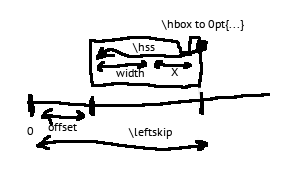
\includegraphics[width=7cm]{calculations.png}

The image reflects how the boxes, glues and lengths are related. We see that \verb|offset|+\verb|width|+\verb|x| is \verb|leftskip|, therefore \verb|x| (\verb|\dimen0|) is \verb|leftskip| minus \verb|offset| minus \verb|width|.

% =========================================================

\section{Paragraph designer referense}

\paragraph{Denomination.} \verb|cmd|, \verb|env|, \verb|stylecmd|. These are the names for the generated commands and environments.

An examples of \verb|cmd| and \verb|env| are already given. The command for \verb|stylecmd| makes a character style, which affects the font and doesn't set the paragraph properties (vertical spacing, tabulars etc).

A sample paragraph definition:

\begin{verbatim}
ParagraphOptions(cmd="Caption,
  stylecmd="UseCaption", ...)
\end{verbatim}

In a \LaTeX{} document you can write:

\begin{verbatim}
{\UseCaption Article 1.} All human beings
are born free and equal in dignity ...
\end{verbatim}

All the three denominators can be mixed together at once. You must specify \verb|cmd| even if you don't need it.

\paragraph{Fonts.} \verb|fontsize|, \verb|baseline|, \verb|fontcmd|.

The only supported font properties are its size and baseline. The rest properties, such as width or serie, should be manually defined in \verb|fontcmd|:

\begin{verbatim}
ParagraphOptions(...,
    fontcmd=r'\fontseries{b}\selectfont',
    ...)
\end{verbatim}

\paragraph{Dimensions.} \verb|leftskip|, \verb|hsize|, \verb|space_above| and \verb|space_below|.

The names are self-explaining.

The default value for \verb|space_above| and also for \verb|space_below| is 0pt. It means that if you haven't given a value, then two consequent paragraphs will touch each other, like if \cs{nointerlineskip} were given between them.

Use the special value \verb|#natural| to disable the use of \cs{ParaSpaceAbove} or \cs{ParaSpaceBelow} and activate instead the default \TeX{} behaviour.

\begin{verbatim}
ParagraphOptions(...,
  space_above='#natural',
  space_below='#natural', ...)
\end{verbatim}

\paragraph{Tuning.} \verb|moresetup|, \verb|afterpar|, \verb|preamble_arg1|, \verb|preamble_arg2|, \verb|preamble_arg3|, \verb|preamble_arg4|.

The content of \verb|moresetup| is literally copied into the style difinition at the end of the paragraph setup, just before \cs{noindent}. A few ideas what can be set in \verb|moresetup|:

\begin{itemize}
\item A color of the paragraph text,
\item \cs{penalty} to suggest a page break,
\item \cs{interlinepenalty} for list item paragraphs, to avoid a page breaks inside.
\end{itemize}

The content of \verb|afterpar| is literally copied into the style definition directly after \verb|{...\par}|. This place is good to put \cs{nobreak} or some other penalty.

The content of \verb|preamble_argN| is copied literally into the style definition directly before \verb|#N|. Possible applications:

\begin{itemize}
\item Add \cs{ignorespaces} if the text might contain spuorious spaces at the beginning.
\item For list item paragraphs, \cs{hfil} centers the tabulator box content, \cs{hfill} aligns to the right.
\end{itemize}

\paragraph{Tabstops.} Tabstops are hboxes of a given width at given offset.

\begin{verbatim}
ParagraphOptions(...,
  boxes=(
    (OFFSET1,WIDTH1),
    (OFFSET2,WIDTH2),
    ...,
    (OFFSETn,WIDTHn)),
  ...)
\end{verbatim}

Due to Python pecularities, one-element list of lists should have an additional comma, otherwise Python unwraps one level of parentheses. The correct way is:

\begin{verbatim}
ParagraphOptions(...,
  boxes=((OFFSET,WIDTH),), # Comma inside
  ...)
\end{verbatim}

All the offsets are relative to the left border of the text flow.

The content of the boxes is left-aligned. To center or right-align the content, add \cs{hfil} or \cs{hfill} through the parameter \verb|preamble_argN|.

\paragraph{Inheritance.} The parameter \verb|parent| uses an already existing paragraph object as the starting point for the paragraph being defined. The properties, which are not specified in the new paragraph definition, are taken from the parent.

\begin{verbatim}
head_i = ParagraphOptions(
    cmd='HeadI',
    fontsize='12pt', baseline='14pt',
    fontcmd=r'\fontseries{b}\selectfont',
    ... )

ParagraphOptions(cmd='HeadII',
    parent=head_i, # Inheritance
    fontsize='11pt', baseline='13pt',
    ... )
\end{verbatim}

In the example, the paragraph \verb|HeadII| inherits \verb|fontcmd| from \verb|HeadI|, but uses the custom font size and baseline.

\paragraph{The infrastructure.} A python file with definitions (1) starts by importing the support code, (2) continues with collecting the definitions and (3) finishes by the command to dump the \TeX{} result.

\begin{verbatim}
from parades import * # 1

add_style(ParagraphOptions(...)) # 2
add_style(ParagraphOptions(...))
...
add_style(ParagraphOptions(...))

main('paras') # 3
\end{verbatim}

The parameter of the function \verb|main| (in this example \verb|paras|) is the name of the generated sty-package as given by \cs{ProvidesPackage}.

% =========================================================

\section{Getting and running the code}

All the files, including the example, are contained in the \acro{CTAN} package \verb|parades|. Alternatevely, one can download it on github or get the sources in the git repository: \url{https://github.com/olpa/tex}, in the folder \verb|parades|.

Put the file \verb|paravesp.sty| into a directory in which \TeX{} will find it. Put the file \verb|parades.py| into a directory in which Python will find it.

The paragraph generator runs from the command line.

\begin{verbatim}
$ python input-defs.py [output-defs.sty]
\end{verbatim}

The script \verb|input-defs.py| is the file with the python definitions of the paragraphs. The optional arguments is the name of the \verb|.sty|-file with the generated \TeX{} definitions. If the output file is not specified, the code is dumped to the standard output.

The directory \verb|udhr| contains a sample project. Refer to the file \verb|README| in this directory for details how to use it.

% =========================================================
\section{Conclusion}

The paragraph designer helps both on the technical and organization levels.
On the technical level, it helps generating code for paragraph styles. Writing this code manually were an unpleasant error-prone task:

\begin{itemize}
\item Space above and below a paragraph.
\item Paragraphs with tabstops such as list items, table of content entries, headers.
\end{itemize}

On the organization level, the python-scripts allow to have a common code base and adapt it to the needs of specific layouts.

The \LaTeX{} package \verb|paravesp| can be used independently of the paragraph designer to implement vertical spacing.

There are problems with the package \verb|paravesp| and the paragraph designer:

\begin{itemize}
\item Many features are not implemented and some need rework.
\item The \LaTeX{} code written in the galley style is too verbose to be typeset manually.
\end{itemize}

The paragraph designer is used in a production system for years. The benefits compensate the problems.

\end{document}
